\chapter{Introduction}


\section{Motivation} % why is this a non trivial problem

Modern social media has entrenched itself as the most accessible and heard voice for the modern digitized populace.
Platforms such as Twitter, Facebook and Youtube allow their users to generate and share opinionated content across the Web.
\citet{Balahur2014} states that this data has proven to be of tremendous value for a whole range of applications, in Economics, Social Science, Political Science and Marketing.
Despite such advantages, the scale of the content in this available data makes it difficult to access and use.
Platforms like Twitter offer a fast and effective \ac{API} that allows researchers to collect and analyze users' content, including opinions on their personal view on the Covid-19 Vaccine.
However less than 1\% of Twitter data is geo-tagged, which means that classifying the origin country of any data gathered is tedious.
Since most online content is generated in English, the use of other languages cannot be ignored as they can be used as indicators for an origin country or region.
For this purpose of geo-localization, newspaper articles are better suited, as it is easier to identify for which country an article is written for.
Progress made in the \ac{NLP} field has made data collection, analyses and evaluation on big data language projects possible.
\ac{SA} has become a popular tool used for automated analyses for large scale and varied language content.


%\begin{figure}[HT!]
%  \centering
%  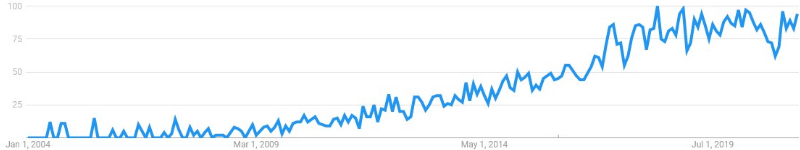
\includegraphics[width=0.6\linewidth]{google.jpg}
%  \caption[Google Trends for \ac{SA} from 2004--2021]{Google Trends for \ac{SA} from 2004--2021.\index{Google Trend}}
%  \label{fig:googletrend}
%\end{figure}

% Maybe not for motivation
%To focus the analyses on European countries and citizens tweets where collected in 6 languages: English, Spanish, French, German, Italian and Dutch.
%The data was collected over a range of 30 dates spanning 6 months from December 2020 till May 2021.
%To diversify the data collected from Twitter 900 articles where also collected that where written about the Covid-19 pandemic.
%Articles where collected for 6 countries: United Kingdom, Spain, France, Germany, Italy, Netherlands, and over the same date range as the Twitter dataset.


\section{Aims and Objectives}

Positive public opinion on the Covid-19 vaccine is essential for an effective vaccine rollout and public or private strategies that are affected by the pandemic.
The aim of this \ac{IAPT} is to collect publicly available opinions on the Covid-19 pandemic, analyze and extract valuable knowledge to present as an explanation to the sentiment change over time.
The effect of Twitter data and publicly available newspaper article headings was investigated for trends and insights.

\noindent A number of objectives were defined in the thesis:

\begin{enumerate}
  \item Collect a sizeable and relevant publicly available dataset from a social media platform that covers a number of European countries.
  \item Collect a sizeable and relevant publicly available dataset from a number of European newspapers that covers a number of European countries.
  \item Preprocess and translate this data so that it can be used as an input for a \ac{SA} model.
  \item Implement a \ac{SA} model to analyze the collected data.
  \item Analyze and extract knowledge from the \ac{SA} scores by visualizing the results.
\end{enumerate}

\section{Summary of Solution Developed}

Using the Twitter \ac{API}~\citep{roesslein2020tweepy} and by manually using the Google search engine to collect a number of articles related to six European countries: the United Kingdom, Spain, France, Germany, Italy and the Netherlands.
A number of Python notebooks were developed to collect, filter, process, analyze and visualize this data and the products of its analyses.
The Google Cloud Translate \ac{API} was used to translate non-English tweet texts to English texts.
A \ac{VADER}~\citep{Hutto_Gilbert_2014} model was used as provided by the \ac{NLTK} library~\citep{bird2009natural}.
Finally the multiplex visualization library~\citep{Mamo2021} was extensively used to visualize the data in its processed and analyzed form.


\section{Document Structure}

Chapter 2 contains a background and review of the relevant literature.
The methods used in the study are then described in Chapter 3, after which the results are presented and discussed in Chapter 4.
Finally, Chapter 5 outlines the main conclusions and identifies both limitations to the study and recommendations for further research.

